\documentclass[../Elmag-labhefte-2020.tex]{subfiles}


\begin{document}

\chapter{ELECTROSTATIC POWER \label{ch.coulomb}}

\subsection*{Goal}

You are going into this lab assignment
%
\begin{itemize}
\item repeat Coulomb's epoch-making experiment from 1785, ie \ measure electrostatic force sfa. \ distance,
\item study the dependence of the electrostatic force on the charge,
\item determine the electrical permittivity of air,
\item keep a thorough journal and perform a thorough error analysis.
\end{itemize}
%


%**********************************************
\section{Theoretical background}
%**********************************************

Here the theory is presented very briefly. Some theory is also reviewed in the text of the calculation tasks in section \ref{ch.coulomb.beregn}. Otherwise, reference is made to the textbook and the lectures in electricity and magnetism.

%**********************************************
\subsection{Coulomb's Law}
%**********************************************

The electrostatic force (Coulomb force) $F_\text{e}$ between two point charges $q_1$ and $q_2$ at a distance $r$ in empty space is given by Coulomb's law:
\begin{equation}
    F_\text{e}
        = \frac{1}{4\pi\epsilon_0} \frac{q_1 q_2}{r^2}
    \label{eq:coulomb}
\end{equation}
where $\epsilon_0 = \SI{8.854e-12}{\farad/\m}$ is the void permittivity.

%**********************************************
\subsection{Force Sensors}
\label{subsec.kraftsensor}
%**********************************************

Coulomb used a torsion scale in his experiment in 1785 \footnote{The operation of a torsion scale was thoroughly reviewed in the experiment for determining the gravitational constant in the lab course in Mechanical Physics, and we therefore refer to the lab booklet in Mechanical Physics for a detailed description and operation.} measure the electrostatic force between two charged metal spheres and thus establish the inverse square ratio of force to distance. It is common to represent deviations from the inverse square law by expressing the distance dependence as $r^{-2\pm q}$. Coulomb's value for $q$ is \num{4e-2}. There have been many attempts to find a more precise value. In 1971, Williams, Faller, and Hill \footnote{\textit{Phys. Rev. Lett.} \textbf{26}, 721 (1971)} examined the validity of Coulomb's law in the most accurate "macroscopic" experiment to date. Given the distance dependence on the shape $r^{-(2+q)}$, they found that $q = \num{2,7\pm3,1e-16}$.

In the experiment, use a force sensor to repeat Coulomb's experiment. Since the power sensor provides a direct measurement value, it is important for us to have an understanding of how this works, and why it states the measurement figures it makes.


%******************************************
\subsubsection{Stretch flap} \vspace{-5mm}
%******************************************
The ohmic resistance of a material of length $l$ and a cross-sectional area $A$ is given by
\begin{equation}
    R = \rho \frac{l}{A},
    \label{eq:R_sfa_lA}
\end{equation}
where $\rho$ is the specific resistance of the material. This can be used to make a tensile sensor, which increases the resistance if the length of a conductor is increased and reduces the resistance correspondingly if the conductor is compressed. The cross-sectional area also decreases somewhat with elongation and increases somewhat with compression. This will, seen from equation \eqref{eq:R_sfa_lA}, be an advantage as we want the largest possible measurable change in the resistance.

A strain gauge sensor is a conductor laid on an elastic foil in such a way that a change in one dimension can be easily detected, while a change in the other dimensions does not significantly affect the sensor. A typical stretch flap is shown in Figure \ref{fig:strekklapp}. Which direction is the sensitive direction for measurements and why?

\begin{figure}[h!b]
    \centering
    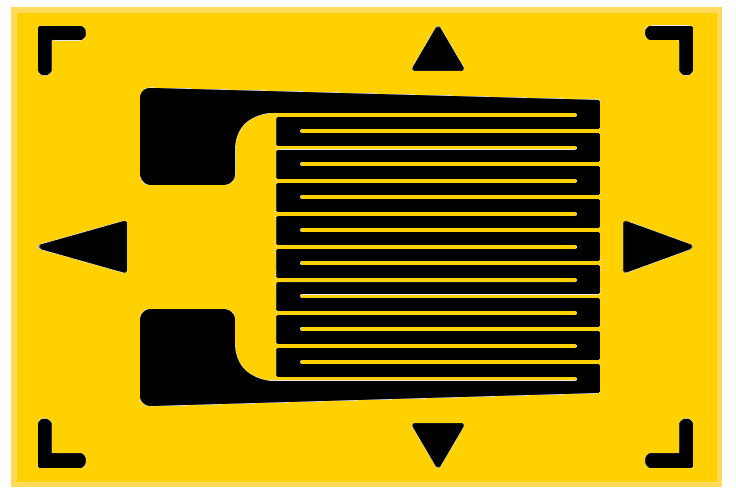
\includegraphics[width=6.01cm,height=3cm,keepaspectratio]{fig/strekklapp.png}
    \caption{%
        En strekklapp er en leder (i svart) lagt på en elastisk folie, her vist i forstørret utgave. Pilene er kun som hjelpemiddel for å plassere strekklappen riktig. De store områdene i enden av lederen er loddepunkter for tilkopling av ledning.
    }   
    \label{fig:strekklapp}
\end{figure}


%******************************************
\subsubsection{Wheatsones bro} \vspace{-5mm}
%******************************************
Wheatstone's bridge, which basically consists of two voltage dividers \footnote{See chapter \ref{lorentz.spenningsdeler} for a repetition / introduction of what a voltage divider is.}, Is a classic and effective way to find the value of an unknown opponent. The bridge consists of a known voltage source, four resistors, and a sensitive measuring instrument (galvanometer or multimeter). Traditionally, such a setup was used to measure the magnitude of an unknown resistor by letting it enter the bridge together with a known resistor and with an accurately variable resistor (sliding resistor) connected for one voltage divider.
In Figure \ref{fig:wheatstonebridge}, typically $R_1$ and $R_2$ would be the shear resistance, $R_3$ would have known value, and $R_4$ would be the unknown resistance. You set the sliding resistance and find when the measuring instrument does not show any deflection. The ratio between the known and unknown resistors is then given by the ratio of the sliding resistor, and one can then calculate the value of the unknown resistor.


\begin{figure}[htbp]
    \centering
    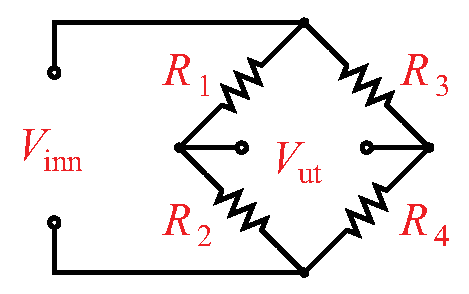
\includegraphics[height=3cm,keepaspectratio]{wheatstonebridge.eps}
    \caption{%
        Klassisk oppstilling av en Wheatstone-bro, med spenningskilde $V_\text{inn}$, fire motstander $R_1$ -- $R_4$, og et målepunkt $V_\text{ut}$.
    }
    \label{fig:wheatstonebridge}
\end{figure}


%******************************************
\subsubsection{Force Sensors} \vspace{-5mm}
%******************************************
In the power sensor itself, the Wheatstone bridge is used a little differently than explained above. Instead of varying the resistances of the output voltage $V_\text{ut} = 0$, only the voltage is read as a measure of how different the resistances are. Four tension flaps are used on a adapted body, positioned so that two are compressed and two are stretched. Figure \ref{fig:ForceSensor} shows a cross section of the force sensor that we use in our experiment. The four tension flaps are identical when the sensor has no load and has a value of $R$, when they are subjected to a load (either tension or compression) we denote the change ${\Delta R}$.

From equation \eqref{eq:R_sfa_lA} we see that a change in resistance in a tensile flap is proportional to a change in its length \footnote{The cross section of the conductor in the tensile flap does not change significantly.}. Furthermore, we can assume that Hooke's law applies to the material in the sensor, ie that a change in length is proportional to the force applied. This means that the change in resistance $\Delta R$ is proportional to the force. It can be shown that the output voltage, $V_\text{ut}$, is proportional to the change in resistance, $\Delta R$, and thus we see that the output voltage of the force sensor is linearly dependent on the force it is to measure \footnote{The relationship between output voltage, $V_\text{ut}$, and change in resistance, $\Delta R$, is given in equation \eqref{eq:fullbridge}. You will arrive at this connection yourself in one of the pre-assignments in chapter \ref{ch.coulomb.beregn}.}.

The power sensor is connected to a `` universal display unit '' which converts the output signal to power measured in \si{\milli\newton}. We cannot change this conversion, the calibration, but it should be checked. The unit has a reset button marked $\rightarrow 0 \leftarrow$, by pressing this the unit uses the current value of the output voltage, $V_\text{ut}$, as the zero reference point for further calculation of power. The power sensor and the electronics of the display unit require a certain warm-up time before it stabilizes. Therefore, be sure to turn on the unit for at least half an hour before taking the actual measuring series to avoid operation. The overall setup for the experiment is shown in Figure \ref{fig:CoulombSetUp_new}.

\begin{figure}[!htbp]
    \centering
    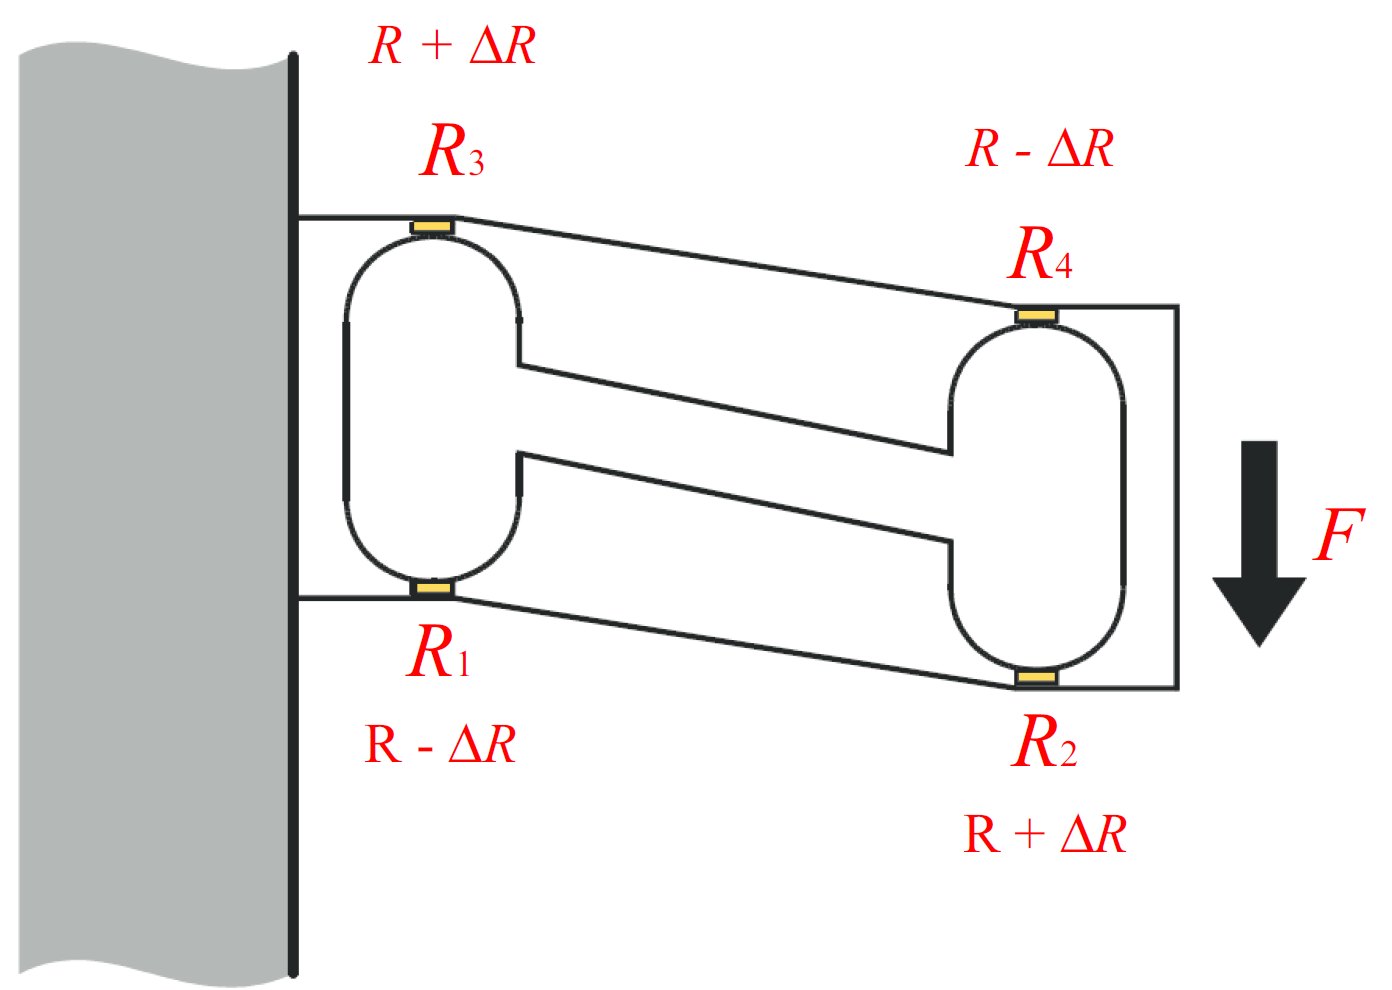
\includegraphics[width=12cm,height=8cm,keepaspectratio]{ForceSensor.png}
    \caption{%
        Tverrsnitt av kraftsensoren som består av et metallstykke med som bøyes i enkelte punkter. Fire strekklapper med lik motstand $R$ er plassert i de punkter hvor metallet har størst påkjenning og resistansen i disse endres med $\Delta R$ ved belastning.
    }
    \label{fig:ForceSensor}
\end{figure}

\begin{figure}[h!t]
    \centering
    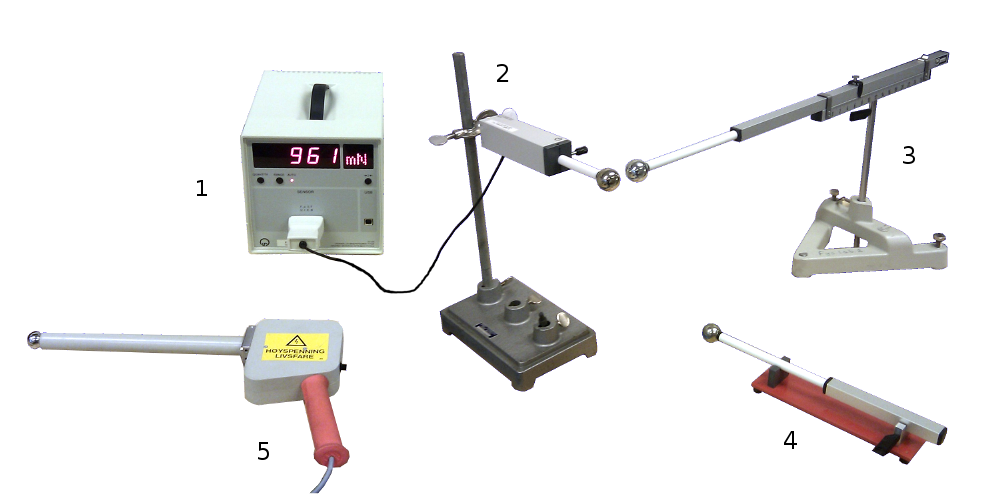
\includegraphics[width=15cm,height=7.5cm,keepaspectratio]{CoulombSetup-new.png}
    \vspace{-2mm}
    \caption{%
        Forsøksoppstillingen i Coulombeksperimentet. 
	        (1) visningsenheten, 
	        (2) kraftsensor med arm og kondensatorkule K\textsubscript{2}, 
	        (3) målestativ med kondensatorkule K\textsubscript{1}, 
	        (4) ladningsøsen med kondensatorkule K\textsubscript{3}, og
	        (5) høyspenningskanonen.
        Faradayburet er ikke vist.
     }
   \label{fig:CoulombSetUp_new}
\end{figure}

\clearpage


%%%%%%%%%%%%%%%%%%%%%%%%%%%%%%%%%%%%%%%%%%%%%%%%%%%
\section{Calculation tasks / preliminary tasks \label{ch.coulomb.beregn}}
%%%%%%%%%%%%%%%%%%%%%%%%%%%%%
\subsection{Wheatstone Bridge}
The setup that the force sensor uses to measure change in resistance is called a full bridge, which we will take a closer look at.

{\itsf 1. Based on Figures \ref{fig:wheatstonebridge} and \ref{fig:ForceSensor}, show that the relationship between the input voltage $V_\text{inn}$ and the output voltage $V_\text{ut}$ is given by the formula}
\begin{equation}
    \label{eq:fullbridge}
    V_\text{ut} = \frac{\Delta R}  {R} V_\text{inn} .
\end{equation}

Tip: Since a voltmeter has a large internal resistance, you can assume that the current through the output is zero. \ \
A typical resting resistance (the resistance without load) for a tensile flap is \SI{120}{\ohm}.


\subsection{Metal ball in empty space}

The ability of an electrode to pick up charge depends, among other things, on of the capacitance of the electrode defined by
\begin{equation}
    C = \frac{q}{V},
    \label{eq:coulomb.3.1}
\end{equation}
where $q$ the charge of the electrode and $V$ the potential (voltage) of the electrode are relatively infinite. For a metal \ sphere with a radius $\rho$, we can calculate from Gauss's law that the capacitance in empty space is
\begin{equation}
    C = 4\pi\, \epsilon_0 \, \rho .
    \label{eq:coulomb.3.2}
\end{equation}
%
In the experiment, use spherical electrodes with radius $\rho = \SI{15}{\milli\m}$.

{\itsf 2A. Calculate the capacitance of such an electrode.}
%Svar: 1,67 pF.

{\itsf 2B. Calculate the charge on the electrode when it is charged to an electrical potential equal to \SI{25}{\kilo\volt}. }
% 20 nC.

\subsection{Determination of charge using. Faradaybur \label{ch.Faradaybur}}
%%%%%%%%%%%%%%%%%%%%%%%%%%%%%

According to Coulomb's law \eqref{eq:coulomb}, there is a repulsive force between equal electric charges. Charges on an electrode will therefore seek as far away from each other as possible and consequently be distributed evenly over the outer surface of the electrode. Inside the electrode it will then be both charge-free and field-free. This was proved by Faraday.
\begin{figure}[!ht]
    \centering
    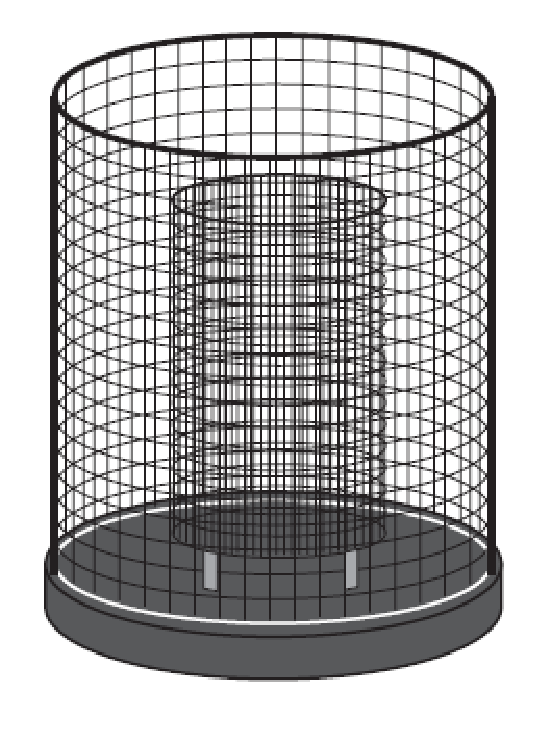
\includegraphics[scale=0.5]{FaradayBur.eps}
    \vspace{-5mm}
    \caption{%
        Faradayburet.
    }
    \label{fig:FaradayBur}
    \vspace{-5mm}
\end{figure}
 
\begin{figure}[!ht]
    \vspace{-2cm}
    \hspace{2cm}
    \setlength{\unitlength}{1mm}
    \begin{picture}(40, 60)(-70,20)       
        \thicklines
        \put(25, 45){\Large\sf C}
        \put(35, 39.5){\circle{6}}
        \put(37, 41.8){\line(1, 1){9.8}}
        \put(37.4, 40.7){\line(1, 1){10}}
        \put(40, 20){\oval(20,10)[b]}
        \put(30, 20){\line(0, 1){25}}
        \put(50, 20){\line(0, 1){25}}
        \put(30, -5){\framebox(20,10)}
        \put(30, 7){\small\sf elektrometer}
        \put(40, 1.75){\oval(16,4)}
        \put(33.5, 0.7){\small\sf 0123456}
        \color{red}
        \put(36, -2.5){\circle{2}}
        \put(36, -2.5){\circle{3}}
        \qbezier(31, 17)(1, 3)(36, -2.5)
        \color{magenta}
        \put(37, 45){\vector(1, 1){9.8}}
        \color{blue}
        \put(44, -2.5){\circle{2}}
        \put(44, -2.5){\circle{3}}
        \put(44, -2.5){\line(0, -1){6}}
        \put(41, -9){\line(1, 0){6}}
        \put(42, -10){\line(1, 0){4}}
        \put(43, -11){\line(1, 0){2}}
        \color{red}
        \put(26, 30){\large$+$}
        \put(26, 35){\large$+$}
        \put(26, 25){\large$+$}
        \put(35, 12){\large$+$}
        \put(41, 12){\large$+$}
        \put(26, 20){\large$+$}
        \put(51, 30){\large$+$}
        \put(51, 35){\large$+$}
        \put(51, 25){\large$+$}
        \put(51, 20){\large$+$}
    \end{picture}
    \begin{picture}(40, 60)(20,20)
        \thicklines
        \put(25, 45){\Large\sf B}
        \put(33, 39.5){\circle{6}}
        \put(35, 41.8){\line(1, 1){9.8}}
        \put(35.4, 40.7){\line(1, 1){10}}
        \put(40, 20){\oval(20,10)[b]}
        \put(30, 20){\line(0, 1){25}}
        \put(50, 20){\line(0, 1){25}}
        \put(30, -5){\framebox(20,10)}
        \put(30, 7){\small\sf elektrometer}
        \put(40, 1.75){\oval(16,4)}
        \put(33.5, 0.7){\small\sf 0123456}
        \color{blue}
        \put(44, -2.5){\circle{2}}
        \put(44, -2.5){\circle{3}}
        \put(44, -2.5){\line(0, -1){6}}
        \put(41, -9){\line(1, 0){6}}
        \put(42, -10){\line(1, 0){4}}
        \put(43, -11){\line(1, 0){2}}
        \color{red}
        \qbezier(31, 17)(1, 3)(36, -2.5)
        \put(36, -2.5){\circle{2}}
        \put(36, -2.5){\circle{3}}
        \put(26, 30){\large$+$}
        \put(26, 35){\large$+$}
        \put(26, 25){\large$+$}
        \put(35, 12){\large$+$}
        \put(41, 12){\large$+$}
        \put(26, 20){\large$+$}
        \put(51, 30){\large$+$}
        \put(51, 35){\large$+$}
        \put(51, 25){\large$+$}
        \put(51, 20){\large$+$}
    \end{picture}
    \begin{picture}(40, 60)(110,20) 
        \thicklines
        \put(25, 45){\Large\sf A}
        \put(35, 39.5){\circle{6}}
        \put(37, 41.8){\line(1, 1){9.8}}
        \put(37.4, 40.7){\line(1, 1){10}}
        \color{red}
        \color{black}
        \put(30, 7){\small\sf elektrometer}
        \put(30, -5){\framebox(20,10)}
        \put(40, 20){\oval(20,10)[b]}
        \put(30, 20){\line(0, 1){25}}
        \put(50, 20){\line(0, 1){25}}
        \put(40, 1.75){\oval(16,4)}
        \put(33.5, 0.7){\small\sf 0123456}
        \color{blue}
        \put(44, -2.5){\circle{2}}
        \put(44, -2.5){\circle{3}}
        \put(44, -2.5){\line(0, -1){6}}
        \put(41, -9){\line(1, 0){6}}
        \put(42, -10){\line(1, 0){4}}
        \put(43, -11){\line(1, 0){2}}
        \color{green}
        \put(44, 54){\vector(-1, -1){9.8}}
        \color{red}
        \qbezier(31, 17)(1, 3)(36, -2.5)
        \put(36, -2.5){\circle{2}}
        \put(36, -2.5){\circle{3}}
        \put(33,38.2){\Large$+$}
        \put(33.1,38.3){\Large$+$}
        \put(32.9,38.1){\Large$+$}
        \put(26, 30){\large$+$}
        \put(26, 35){\large$+$}
        \put(26, 25){\large$+$}
        \put(35, 12){\large$+$}
        \put(41, 12){\large$+$}
        \put(26, 20){\large$+$}
        \put(51, 30){\large$+$}
        \put(51, 35){\large$+$}
        \put(51, 25){\large$+$}
        \put(51, 20){\large$+$}
        \color{blue}
        \put(31, 30){\large$-$}
        \put(31, 35){\large$-$}
        \put(31, 25){\large$-$}
        \put(35, 16){\large$-$}
        \put(41, 16){\large$-$}
        \put(31, 20){\large$-$}
        \put(46, 30){\large$-$}
        \put(46, 35){\large$-$}
        \put(46, 25){\large$-$}
        \put(46, 20){\large$-$}
    \end{picture}
    \vspace{3cm}
    \caption{%
        Måling av ladning med Faradaybur og elektrometer. Faradayburet er isolert fra jord og potensialet relativt jord måles. A: Ladd elektrode føres inn i Faradayburet og elektrometeret viser umiddelbart utslag. B: Elektroden i kontakt med Faradayburet. C: Elektroden trekkes ut og elektrometeret viser fortsatt samme utslag. Elektrodens opprinnelige ladning er overført til Faradaybur/ledning/elektrometer.
    }
    \label{fig:FaradayExpt}
\end{figure}
Faraday electrically insulated a metal bucket and connected an electroscope to the outside of the bucket. Then he lowered a loaded metal ball, where the ball was fastened in a silk thread (which is a good insulator), into the bucket. As the ball came in contact with the bottom, the electroscope showed that the bucket changed state from uncharged to charged. The electroscope also showed results before the ball was in physical contact with the bucket, and when the ball was taken up by the bucket, examinations showed that it was uncharged. Faraday interpreted this so that when the bullet touches the bottom of the bucket and becomes part of it, electrically speaking, the charges (which were originally placed on the outside of the bullet) will move to the outside of the bucket.

We can use Faraday's setup to measure the charge on a charged electrode: The Faraday cage is shown in Figure \ref{fig:FaradayBur} and the setup is shown in Figure \ref{fig:FaradayExpt}. The electrode with the charge to be measured is immersed in the hollow electrode, the so-called Faraday cage, which is well isolated from earth and corresponds to the bucket in Faraday's experiment. Instead of an electroscope, we use an electrometer to measure the voltage $V_\text{f}$ of the Faraday cage relative to the earth.


The Faraday cage, the wires of the electrometer and the electrometer itself can be considered as an electrode configuration that has a certain constant capacitance $C = C_\text{Faradaybur} + C_\mathrm{ledninger} + C_\text{elektrometer}$ to ground. If this capacitance is known (or it can be measured), the charge can be calculated from $q = C V_\text{f}$.

Assume that $C = \SI{130}{\pico\farad}$ and that a voltage $V_\text{f} = \SI{60}{\volt}$ is measured when a particular charged electrode is lowered into the Faraday cage.

{\itsf 3. Calculate the charge $q$ on the electrode.}
% Svar: 7,8 nC.

The Faraday cage itself is isolated from earth, but surrounded by a grounded mesh cylinder that shields against electromagnetic noise. A coaxial cable (see Figures \ref{fig:CoaxCable} and \ref{fig:BNC03})

\begin{figure}[!h]
    \begin{minipage}[b]{0.5\linewidth}
        \centering
        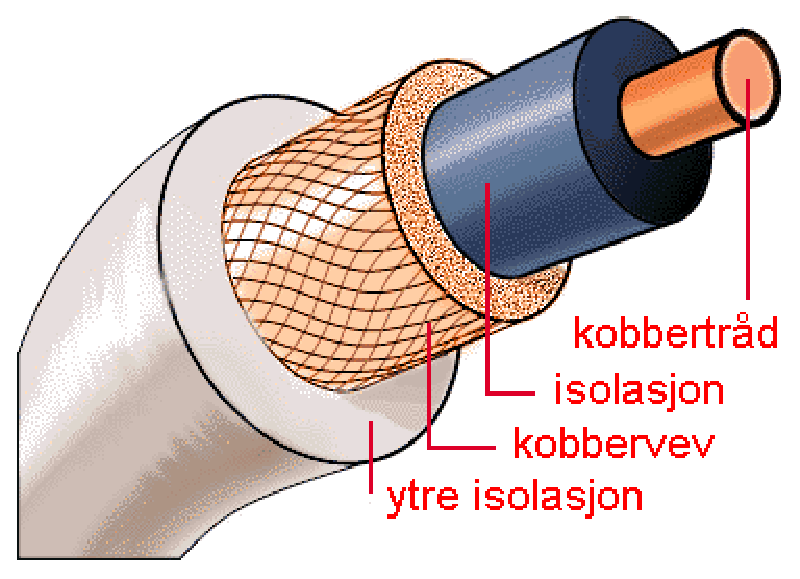
\includegraphics[scale=0.45]{CoaxCable.eps}
        \caption{%
            Tverrsnitt av en koaksialkabel.
        }
        \label{fig:CoaxCable}
    \end{minipage}
    \hspace{0.15cm}
    \begin{minipage}[b]{0.5\linewidth}
        \centering
        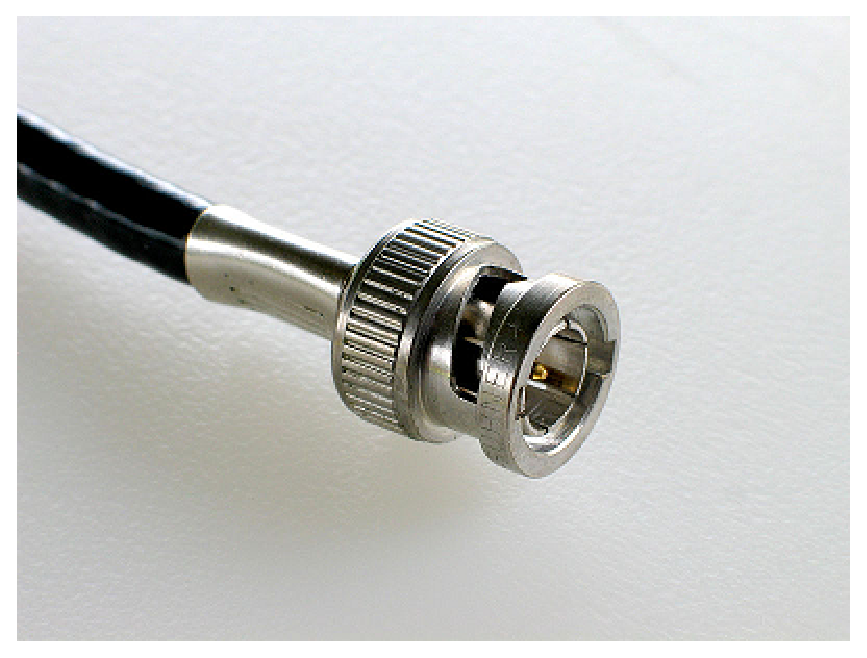
\includegraphics[width=6cm,height=4.5cm,keepaspectratio]{BNC03.eps}
        \caption{%
            Koaksialkabel med BNC-tilkopling.
        }
        \label{fig:BNC03}
    \end{minipage}
\end{figure}
is connected to the electrometer. This cable has two terminals, of which the center conductor is connected to the Faraday cage and the shield wire to the surrounding mesh cylinder. This is outlined in Figure \ref{coulomb.fig1b}. In addition, a ground wire is connected from the ground point of the electrometer to the ground shield. The electrometer measures the voltage between the input terminals by connecting the voltage across a known, large resistance $R_\text{i}$ between the input terminals, and measuring the current $I$ in the resistor. From Ohm's law, the voltage $V_\text{f} = R_\text{i}  I$ is calculated, and the scale of the electrometer shows the voltage $V_\text{f}$ directly.

\begin{figure}[!h]
    \vspace{-1cm}
    \hspace{2cm}
    \setlength{\unitlength}{0.8mm}
    \begin{picture}(40, 60)(-50,20)        
        \thicklines
        \put(40, 20){\oval(20,10)[b]}
        \put(30, 20){\line(0, 1){25}}
        \put(50, 20){\line(0, 1){25}}
        \multiput(15,-4)(0,6){10}{\line(0, 1){5}}
        \multiput(65,-4)(0,6){10}{\line(0, 1){5}}
        \put(31, 0){\oval(16,8)[br]}
        \put(49, 0){\oval(16,8)[bl]}
        \put(39, 0){\line(0, 1){15}}
        \put(41, 0){\line(0, 1){15}}
        \put(-30, -5){\framebox(30,22)}
        \qbezier(-23, 9)(-16, 12)(-9, 9)
        \qbezier(-25, 12)(-16, 15)(-7, 12)
        \qbezier(-25, 12)(-24, 11)(-23, 9)
        \qbezier(-9, 9)(-8, 11)(-7, 12)
        \qbezier(-14, 10.5)(-13, 12)(-12, 13)
        \put(-25, -1){\circle{2}}
        \put(-25, -1){\circle{3}}
        \put(-20, -1){\circle{2}}
        \put(-20, -1){\circle{3}}
        \put(-17.5, -2.5){\small\sf GND}
        \put(25, -10){\sf jordingsplate}
        \put(55, 58){\sf jordingsskjerm}
        \put(38, 48){\sf Faradaybur}
        \put(42, 8){\sf isolerende}
        \put(42, 3){\sf fot}
        \put(-4, 12){\circle{2}}
        \put(-4, 12){\circle{3}}
        \put(-4, 7){\circle{2}}
        \put(-4, 7){\circle{3}}
        \put(-4, 2){\circle{2}}
        \put(-4, 2){\circle{3}}
        \linethickness{0.4mm}
        \qbezier(-20, -1)(-12, -12)(12, -5)
        \linethickness{1.5mm}
        \qbezier(-25, -1)(-55, 16)(-5, 52)
        \linethickness{0.4mm}
        \qbezier(-5, 52)(6, 58)(15, 40)
        \qbezier(-5, 52)(24, 72)(30, 45)
        \put(30, 45){\circle{1.5}}
        \put(15, 40){\circle{1.5}}
        \linethickness{1mm}
        \put(10, -4.5){\line(1, 0){60}}
    \end{picture}
    \vspace{3cm}
    \caption{%
        Faradaybur med omgivende skjerm og elektriske koplinger.
    }
    \label{coulomb.fig1b}
\end{figure}

The charge supplied to the electrometer for measurement will thus leak to earth through $R_\text{i}$. The resistance $R_\text{i}$ must therefore be selected large, otherwise the charge will disappear before you can measure it. It can also not be selected too large, as the current $I$ becomes too small to be measured accurately.

Assume that $R_\text{i} = \SI{e14}{\ohm}$, $V_\text{f} = \SI{60}{\volt}$ and $q$ are as calculated above.

{\itsf 4. Estimate how much of the charge leaks to earth through the electrometer in five minutes.}
Catalog \ \
Help: Complete the estimate by assuming that $V_\text{f}$ is approximately constant over five minutes.

{\itsf 5. Is the assumption of constant $V_\text{f}$ reasonable?}
% I = V_f / R = 0,6 pA.  q = It = 180 pC.  (2,3% av 7,8 nC)

Catalog \emph{Sikkerhet med elektrometeret:} \ \
The electrometer can measure voltages up to a maximum \SI{100}{\volt}. Significantly higher voltages will damage the electrometer. Since the input resistance is as large as \SI{e14}{\ohm}, this means. that input currents significantly greater than $I = V/R = \SI{100}{\volt} / \SI{e14}{\ohm} = \SI{e-12}{\ampere} = \SI{1}{\pico\ampere}$ will damage the electrometer.

Your body and clothes are easily charged up to several thousand volts e.g. during a brisk march along the corridor. If you are charged and touch the input terminals of the electrometer, there is a high probability that you will exceed both the current and voltage limits of the electrometer and damage the input circuit. Before you start working with the electrometer, it is therefore important that you discharge your body. What you do \emph{ved å legge begge hender på den jordede skjermplaten som ligger på arbeidsbenken.} During the measurements, keep yourself discharged by letting one hand be in contact with the screen plate as much as possible.

The connection to the electrometer is through a so-called BNC connector. This connector is specially made for use with so-called coaxial cables. Coaxial cables are two conductors where one conductor forms a cylindrical sheath around the other conductor. The cylindrical sheath is used as an earth conductor and at the same time shields the inner conductor from electromagnetic noise.


The Faraday cage consists of a \SI{12}{\cm} deep mesh cylinder with \SI{8}{\cm} diameter, closed at the bottom and isolated from the foot plate with a \SI{5}{\cm} long ceramic rod. Do not touch the ceramic stick with your fingers! Around the Faraday cage, a mesh cylinder is placed which is connected to earth to shield the Faraday cage from electromagnetic noise.

\emph{Fremgangsmåte for måling av ladning (se også avsnitt \ref{ch.Faradaybur}):}
\vspace{-4mm}
\begin{itemize}
    \item Check that the screen plate is earthed and touch the plate with both hands to discharge yourself. Then make sure to hold one hand as much as possible on the screen.
    \item Resetting the electrometer:
    \vspace{-2mm}
    \begin{itemize}
        \item Leave the electrometer switched off with the ZERO button in the "ZERO LOCK" position. Then the input on the electrometer is added to the GND socket on the electrometer.
        \item Set the function switch to \SI{100}{\volt} and switch on the electrometer.
        \item Adjust the zero point with the ZERO-ADJUST button, first with the function selector in position \SI{100}{\volt}, then with the function selector in position \SI{10}{\volt}. Catalog \ \
        NOTE: The electrometer's display instrument only shows the correct value when it is horizontal, so do not raise the instrument.
        \item Set the function selector to position \SI{100}{\volt}.
        \item Switch the ZERO button to the "PUSH TO ZERO" position. By pressing the ZERO button, the Faraday cage is discharged towards the ground potential.
    \end{itemize}

\subsection{Coulombs Law \label{ch.coulomb.beregn.coulomb}}
%%%%%%%%%%%%%%%%%%%%%%%%%%

Assume that you have two spheres with radius $\rho = \SI{15}{\milli\m}$, center-to-center-distance \SI{10}{\cm} and that you place both on an electric potential equal to \SI{25}{\kilo\volt} relatively infinite.

{\itsf 6. What is the electrostatic force between the spheres? Will there be attraction or repulsion?}

%I 7A og 7B: Regn ut verdier for $F_\text{e}$ i området $3\;{\rm cm} \leq r \leq 15\; {\rm cm}$.

{\itsf 7A. Sketch a graph of the force $F_\text{e}$. depending on the distance between the spheres.} Try different options for the x-axis (for example, linear or square).
%Hjelp: Kurva er lineær og og går gjennom origo.

{\itsf 7B. Find ten values   for $r$ that will be \ae evenly distributed against $1/r^2$ \ /} ($\SI{3}{\cm} \leq r \leq \SI{15}{\cm}$)

%{\itsf 7B. Marker en $r$-akse parallelt med $1/r^2$-aksen i diagrammet -- og vis $r$-verdiene som tilsvarer de valgte skalastrekene på $1/r^2$-aksen.}
%\\ Hjelp: $r$-aksens skalainndeling blir selvfølgelig ikke-lineær.

Strictly speaking, Coulomb's law only applies to point charges. For spheres of finite extent, the interaction between the surface charges on the spheres will give an uneven charge distribution on the sphere surfaces. For two spheres with a radius $\rho = \SI{15}{\milli\m}$ at a distance greater than 10 cm, this will lead to a deviation of less than \SI{1}{\percent} in relation to values   calculated using Coulomb's Law \eqref{eq:coulomb}. How big an error does this lead to in the measurements?


\subsection{Gravitational force}

We want to measure the electrostatic force between the spheres with as much accuracy as possible. In the setup, we will have a gravitational interaction between the spheres in addition to the electrostatic force. The bullets weigh about \SI{25}{\g} each. Are the gravitational forces relevant to your measurements?

%{\itsf 8. Beregn gravitasjonskraften mellom kulene. Er det nødvendig å ta hensyn til gravitasjonskraften mellom kulene?}
% 4,2 pN => << 7,8 nC
 
\clearpage


%%%%%%%%%%%%%%%%%%%%%%%%%%%%%%%%%%%%%%%%%%%%%%%%%%
\section{Experimental}
%%%%%%%%%%%%%%%%%%%%%%%%%%%%%%%%%%%%%%%%%%%%%%%%%%

%%%%%%%%%%%%%%%%%%%%%%%%%%%%%%%%%%%%%%%%%%%%%%%%%%
\subsection{Equipment}
%%%%%%%%%%%%%%%%%%%%%%%%%%%%%%%%%%%%%%%%%%%%%%%%%%

The following instruments are included in the line-up:
\vspace{-4mm}
\begin{itemize}
    \item \textbf{Kraftsensor} Leybold S 524 060. Measuring error: $< 1\%$
Resolution: $< 0.01 mN$
    w / accessories:
    \vspace{-2mm}
    \begin{itemize}
        \item \textbf{Visningsenhet}, Leybold UMI 531 835.
        \item \textbf{Arm med kule}, ball diameter \SI{30}{\milli\m}.
        \item \textbf{kalibreringslodd}, weights with carefully measured masses.
    \end{itemize}
    \item \textbf{Høyspenningskanon} Emco DX250. Output voltage / current: \SI{25}{\kilo\volt} / \SI{75}{\micro\ampere}. Input voltage: + \SI{12}{\volt} $\pm \SI{5}{\percent}$.
    \item \textbf{Spenningskilde} EA-PS 2012-05 for high voltage gun, voltage: \SI{12}{\volt}.
    \item \textbf{Ladningsøse}, ball diameter \SI{30}{\milli\m}.
    \item \textbf{Målestativ med kule}, ball diameter \SI{30}{\milli\m}.
    \item \textbf{Diverse utstyr.} Measuring rod \SI{1}{\m}; gauge 0-2 \si{\m}; calipers; spirit level; level w / clamp, plastic gloves.
    Catalog \item \textbf{Faradaybur, elektrometer og tilhørende utstyr:}
    \vspace{-2mm}
    \begin{itemize}
        \item \textbf{Skjermet Faradaybur}, Pasco Mod. ES9058.
        \item \textbf{Elektrometer} w / connection cables. Catalog \ \
              Measuring range: 0- \SI{100}{\volt}, input resistance: $R_\text{i} = \SI{e14}{\ohm}$.
        \item Faraday cage, cable and electrometer have a total capacitance of $C = \SI{130}{\pico\farad}$.
        \item \textbf{Multimeter} Escort EDM168A, 3 digits, or equivalent.
    \end{itemize}
\end{itemize}

%%%%%%%%%%%%%%%%%%%%%%%%%%%%%%%%%%%%%%%%%%%%%%%%%%
\subsection{Precautions}
%%%%%%%%%%%%%%%%%%%%%%%%%%%%%%%%%%%%%%%%%%%%%%%%%%

Catalog \textbf{Høy spenning.} \ \
The high voltage cannon used to charge the bullets provides \SI{25}{\kilo\volt} when activated. However, the current is limited to \SI{75}{\micro\ampere}. Such currents usually have no physiological effect on the body, but still: \emph{Behandle kanonen som om den var livsfarlig.}

Catalog \textbf{Kraftsensoren.} \ \
The power sensor is a precision instrument that you must handle carefully. This is especially true by not exposing it to forces greater than $\pm \SI{2.5}{\newton}$, which can lead to overload of the sensor. The sensor is not intended for measuring forces greater than $\pm \SI{1}{\newton}$.


Catalog \textbf{Isolatorer.} \ \
The surface of the insulators on which the balls are mounted should not be touched with your fingers. Grease and acid from fingerprints will form conductive channels on the surface and reduce the insulation capacity and lead to leakage of charge from the spheres. Use plastic gloves when handling the balls or insulators.


%%%%%%%%%%%%%%%%%%%%%%%%%%%%%%%%%%%%%%%%%%%%%%%%%%
\subsection{Calibration: Verification of the power sensor.}
%%%%%%%%%%%%%%%%%%%%%%%%%%%%%%%%%%%%%%%%%%%%%%%%%%

The power sensor has already been calibrated from Leybold GmbH. We do not know if what it shows is true, and this should be verified.
Set up the force sensor so that it can measure in the vertical direction, make sure that it is plumb and that the sensor is reset.
 
Make measurements with different masses and present this in a graph, force as a function of mass. Estimate slope and uncertainty for this graph.


%%%%%%%%%%%%%%%%%%%%%%%%%%%%%%%%%%%%%%%%%%%%%%%%%%
\subsection{Mounting of ball electrode and preparation of power sensor}
% og dempningsror}
%%%%%%%%%%%%%%%%%%%%%%%%%%%%%%%%%%%%%%%%%%%%%%%%%%

The force sensor must be leveled so that it acts in the horizontal direction for the subsequent experiments. Furthermore, the ball K \textsubscript{2} must be mounted on the ball arm and the force sensor must be reset. A reset check should be done frequently.

Always wear plastic gloves when you have to touch the balls or ball arms.


%%%%%%%%%%%%%%%%%%%%%%%%%%%%%%%%%%%%%%%%%%%%%%%%%%
\subsection{Electrical wiring}
%%%%%%%%%%%%%%%%%%%%%%%%%%%%%%%%%%%%%%%%%%%%%%%%%%
Always try to use the correct color coding on the different wires when setting up an experiment, this makes troubleshooting much easier.

\subsubsection{Connecting electrical wiring:}

\vspace{-4mm}
\begin{itemize}
    \item Connect the high voltage gun to the power supply: Wire with red plug to + \SI{12}{\volt}, blue with black end plug to \SI{0}{\volt}, yellow to ground contact.
    \item \SI{0}{\volt} on the power supply must be earthed reference, therefore connect the earth contact and the \SI{0}{\volt} socket on this.
    \item Connect ground wires to the force sensor stand with ball K \textsubscript{2}, the measuring stand with ball K \textsubscript{1}, the charging ladle with ball K \textsubscript{3}.
\end{itemize}

The device is now ready for use. Ask the lab supervisor to demonstrate the use of the cannon before using it.



%%%%%%%%%%%%%%%%%%%%%%%%%%%%%%%%%%%%%%%%%%%%%%%%%%
\subsection{Experiment 1: Kraft sfa. distance}
%%%%%%%%%%%%%%%%%%%%%%%%%%%%%%%%%%%%%%%%%%%%%%%%%%
 
Task: \ \
{\itsf Undersøk hvordan den elektrostatiske kraften mellom de ladde metallkulene K\textsubscript{1} and K \textsubscript{2} vary as a function of center-to-center distance $r$.
}

Ball K \textsubscript{2} is mounted on the force sensor and ball K \textsubscript{1} is mounted on a sliding arm so that the distance between the balls can be adjusted.


\subsubsection{Analysis of measurement results.}
\vspace{-4mm}
\begin{itemize}
    \item Draw a curve of the force $F_\text{e}$ sfa. $1/r^2$ on graph paper or in Excel / Python. Estimate a trend line.
    \item Calculate the mean and standard deviation for each measured $r$ value based on the different measurement series.
    \item Do your results agree with Coulomb's law? Can you explain any discrepancies? What happens when $r$ is less than 5- \SI{6}{\cm}?
\end{itemize}


While measuring, the charge will gradually leak out of the spheres, especially if you spend a long time on the measuring series. Therefore, try to reduce the time as much as possible but maintain accuracy. Since the premise is that the charge on the spheres must be constant during each measuring series, the charge loss will lead to a measuring error. It is important to set up the measurement procedure so that this source of error can be checked. You can therefore take \emph{flere måleserier} with discharge and charging of the spheres between each series. In the first series you measure (as described) $F_\text{e}$ for decreasing values   of $r$ and in the next series you measure $F_\text{e}$ for the same $r$ values   in ascending order. Comparison of the measurements at corresponding distances between the two series will provide information on changing the charge. Another way to control charge loss is to perform a control measurement at a specific $r$ value e.g. $r = \SI{10}{\cm}$ between each measurement. As long as the result of the control measurement remains constant, you have not lost charge. Even if you notice that the charge is starting to leak, you can continue the measurement, as systematic errors are part of how accurate we can make these measurements.

Another measurement error is that when ball K \textsubscript{2} is displaced as a result of the repulsion, the distance between the balls is not equal to what the scale indicates. This is most important when the bullets are close, but this effect is quite small in our experiment, as it is a matter of small forces and the force sensor does not move far. Make an estimate, if possible of how far the sensor moves at full force between the balls and the small distance.

A third measurement error is due to polarization of the charge on the spheres. Equal charges repel each other so that the center-to-center distance of the charge distribution on each sphere is greater than the geometric center-to-center distance of the spheres. This error is also most significant when the bullets are close. Make an estimate of the size of the error.

What will happen if the bullets do not have the same charge?



%%%%%%%%%%%%%%%%%%%%%%%%%%%%%%%%%%%%%%%%%%%%%%%%%%
\subsection{Experiment 2: Kraft sfa. charge}
%%%%%%%%%%%%%%%%%%%%%%%%%%%%%%%%%%%%%%%%%%%%%%%%%%

Task: \ \
{\itsf Undersøk hvordan den elektrostatiske kraften avhenger av ladningen $q_1$ til kule K\textsubscript{1}. Ie. target The force on bullet K \textsubscript{2} sfa. the charge on sphere K \textsubscript{1}.}

Find an opportunity to reduce the charge on the sphere in a controlled way and set up a series of measurements based on it. Repeat the measurement series several times.

\subsubsection{Analysis of measurement results.}

\vspace{-4mm}
\begin{itemize}
    \item Draw a curve of the force $F_\text{e}$ sfa. charge $q_1$ on graph paper or in Excel / Python. Estimate a trend line.
    \item Calculate the mean and standard deviation for each $q_1$ value.
    \item Do your results agree with Coulomb's law? Can you explain any discrepancies?
\end{itemize}

%http://fcit.usf.edu/network/chap4/chap4.htm
%http://www.google.no/imgres?imgurl=http://www-ece.rice.edu/~jdw/figs/bnc_t.jpg&imgrefurl=http://www.ece.rice.edu/~jdw/unilab.new/file.3.html&h=260&w=327&sz=9&tbnid=4AP2rDHWMwwVdM:&tbnh=94&tbnw=118&prev=/images%3Fq%3DBNC%2Bconnector%2Bsite:.edu&hl=no&usg=__RIEFn0MtcJl4U5WJ9Sm1R_qSZck=&ei=vJ3JSuPLBdPJ-Qby79hH&sa=X&oi=image_result&resnum=4&ct=image

%%%%%%%%%%%%%%%%%%%%%%%%%%%%%%%%%%%%%%%%%%%%%%%%%%
\subsection{Experiment 3: Electrical permittivity}
%%%%%%%%%%%%%%%%%%%%%%%%%%%%%%%%%%%%%%%%%%%%%%%%%%

Task: \ \
{\itsf Du skal beregne verdi for luftas permittivitet $\epsilon_0$ ved to ulike metoder:

\vspace{-4mm}
\begin{itemize}
    \item [I)] Measurement of charge and force on a bullet and application of Coulomb's law \eqref{eq:coulomb}.
    \item [II)] Calculation of the capacitance of a sphere via charge measurement and the assumption of capacitance for a sphere in equation \eqref{eq:coulomb.3.2}.
\end{itemize}
}

\textbf{\emph{Metode I:}}

In Experiment 1, you measured the electrostatic force $F_\text{e}$ between two metal spheres. If you also measure the charge on the spheres, you can from Coulomb's law \eqref{eq:coulomb} determine the permittivity of the air $\epsilon_0$ when the distance is known. Charge measurement can be done by Faradaybur and electrometer, as explained below, with reference to section \ref{ch.Faradaybur}.


%
    \item Determination of charge on sphere K \textsubscript{3} (charge ladle):
    \vspace{-2mm}
    \begin{itemize}
        \item Charge bullet K \textsubscript{3} with the high voltage cannon.
        \item Move the ball to the inside of the Faraday cage to measure the voltage at the Faraday cage.
        \item Repeat the measurement several times to obtain statistical deviations.
        \item Also test the time stability of the measured voltage. Is the voltage stable? If not, what is the reason and how can one take it into account?
        \item After measuring, set the ZERO switch to the "ZERO LOCK" position and switch off the electrometer.
        \item Calculate the charge on the sphere. Assume that the Faraday cage, cable and electrometer have total capacitance $C = \SI{130}{\pico\farad}$.
%Verdien er funnet fra oppgitt inngangskapasitans på $C =$ 30 pf for elektrometeret og målt kapasitans for kabelen, og du kan etterprøve verdien for kabelen vha. multimeteret. 
    \end{itemize}
\end{itemize}

You may have noticed that the electrometer got the final turn even before you touched the grid? This is called induction and is due to the fact that the charge on the sensor attracts / repels the electrons in the grid so that a charge is collected on the outside of the grid that is as large as the charge we want to measure.

Use the result for an optional value of $r$ from Experiment 1 to find the force between two fully charged, well-known spheres. The spheres K \textsubscript{1} and K \textsubscript{2} have the same dimension as the sphere K \textsubscript{3} on the charge axis, so that they are expected to receive the same charge when charged from the electron gun. Remember to halve the charge on K \textsubscript{3} before measuring in the Faraday cage.

{\itsf Calculate air permittivity $\epsilon_0$ with uncertainty from Coulomb's law in equation (\ref{eq:coulomb}).}

\textbf{\emph{Metode II:}}

When the charge is measured and the potential is known, you can calculate the ball's capacitance from equation \eqref{eq:coulomb.3.1}. If the radius of the sphere, $\rho$, is measured, you can calculate the permittivity of the air from the expression \eqref{eq:coulomb.3.2} for the capacitance of the sphere.

Assume that the high voltage cannon charges up to \SI{25}{\kilo\volt} and use that the high voltage cannon and the bullet have the same potential at charge transfer to calculate the capacitance of the bullet.

{\itsf   Calculate air permittivity $\epsilon_0$ with uncertainty from calculated capacitance and use of equation \eqref{eq:coulomb.3.2}.}

\subsubsection{Talk:}
\begin{itemize}
    \item Compare the value of the measured ball capacitance with the calculated value in calculation problem 2A.
    \item Discuss any discrepancies between the measured and calculated value of the capacitance.
     \item Compare your achieved value for $\epsilon_0$ with table value.
    \item What is the agreement with the estimate for $\epsilon_0$ with the two calculation methods? Which value has the least error? Justify your answer.
    \item Is there a correspondence between the measured value and the table value for $\epsilon_0$ within the estimated error limits?
    \item If something deviates, give a reason why.
\end{itemize}


%%%%%%%%%%%%%%%%%%%%%%%%%%%%%%%%%%%%%%%%%%%%%%%%%%%
%\subsection{Diskusjon}
%%%%%%%%%%%%%%%%%%%%%%%%%%%%%%%%%%%%%%%%%%%%%%%%%%%
%
%\begin{itemize}
%\item Sammenlikn måleresultatene fra de ulike deler av eksperimentet.
%\item Diskuter eventuelle uoverenstemmelser. 
%\item Diskuter styrkeforholdet mellom elektrostatisk kraft og gravitasjonskraft.
%\item Diskuter mulige anvendelser av de fysiske effekter som er tatt opp til observasjon i eksperimentet.
%\end{itemize}


%%%%%%%%%%%%%%%%%%%%%%%%%%%%%%%%%%%%%%%%%%%%%%%%%%
\subsection{Closing}
%%%%%%%%%%%%%%%%%%%%%%%%%%%%%%%%%%%%%%%%%%%%%%%%%%
\emph{La kraftmåleren stå påslått}, disconnect the other wires and leave the space in at least as good an order as you found it.

\end{document}

